\documentclass{article}

\usepackage[margin=2.5cm]{geometry}

\usepackage[utf8]{inputenc}

\usepackage{enumitem}
\usepackage{tabularx}
\usepackage{graphicx}
\usepackage{fancyhdr}
\usepackage{fancyvrb}
\usepackage{amsmath}
\usepackage{tcolorbox}
\usepackage{float}
\usepackage{listings}  
\usepackage{xcolor}
\usepackage{subfigure}
\usepackage[htt]{hyphenat}

\definecolor{codegreen}{rgb}{.2,0.6,0}
\definecolor{codegray}{rgb}{0.5,0.5,0.5}
\definecolor{codepurple}{rgb}{0.58,0,0.82}
\definecolor{codeblue}{rgb}{0,0.4,0.82}
\definecolor{codeorange}{rgb}{0.94,0.34,0.0}
\definecolor{backcolour}{rgb}{0.95,0.95,0.92}
\definecolor{backcolourgray}{rgb}{0.92,0.92,0.92}
\definecolor{codewhite}{rgb}{1,1,1}

\lstdefinestyle{mystyle}{
    backgroundcolor=\color{backcolourgray},   
    commentstyle=\color{codegreen},
    keywordstyle=\color{codeblue},
    numberstyle=\tiny\color{black},
    stringstyle=\color{codeorange},
    basicstyle=\ttfamily\footnotesize,
    breakatwhitespace=false,         
    breaklines=true,                 
    captionpos=b,                    
    keepspaces=true,                 
    %numbers=left,                    
    numbersep=5pt,                  
    showspaces=false,                
    showstringspaces=false,
    showtabs=false,                  
    tabsize=2,
    extendedchars=true,
    frame=single
    %, basicstyle=\footnotesize
}
\lstset{style=mystyle}

\usepackage{hyperref}
\hypersetup{
    colorlinks=true,
    linkcolor=blue,
    filecolor=magenta,      
    urlcolor=cyan,
}

\pagestyle{fancy}
\fancyhf{}
\rhead{Arquitectura de ordenadores. Practice 4.}
\lhead{Pablo Cuesta Sierra, Álvaro Zamanillo Sáez}
\cfoot{\thepage}

\usepackage{titlesec}
\titleformat*{\subsection}{\normalsize\bfseries\itshape\color{darkgray}}
\titleformat*{\subsubsection}{\normalsize\itshape\color{darkgray}}

%\setlength{\parskip}{0.15cm}


%parameters: file, caption, label, scale
\newcommand{\myFigure}[4]{%
    \begin{figure}[!ht]
        \includegraphics[width=#4\textwidth]{#1}
        \centering
        \caption{#2}
        \label{#3}
    \end{figure}
}
%grey item for enumerate
\renewcommand{\thesubsubsection}{(\thesubsection.\alph{subsubsection})}
\setcounter{secnumdepth}{4}
\newcommand{\question}[1]{\subsection{#1}}
\newcommand{\subquestion}[1]{\subsubsection{#1}}


\setcounter{section}{-1}
\setcounter{tocdepth}{1} % only sections in the table of contents


\begin{document}


\title{\textbf{Arquitectura de ordenadores. Practice 4.}}
\author{\textbf{Pablo Cuesta Sierra, Álvaro Zamanillo Sáez}\\(group 1392, team 04)}
%\date{}
\maketitle

\begin{tcolorbox}
\tableofcontents
\end{tcolorbox}


\newpage
\section{Exercise 0: Information about the system topology}

We have used the lab computers, which have 6 cores, with hyperthreading not activated. (This is because in the file \emph{/proc/cpuinfo} the number of pysical cores is the same as the number of virtual cores, which is 6).

For the bigger tests, we used the \emph{MV} machine from the cluster; it has 8 cores, we already mentioned this in last practice (3), exercise 0.

%%%%%%%%%%%%%%%%%%%%%%%%%%%%%%%%%%%%%%%%%%%%%%%%%%%%%%%%%%%%%
\section{Exercise 1: Basic OpenMP programs}

\question{Is it possible run more threads than cores on the system? Does it make sense to do it?}

It is possible to do so: if we first execute omp1 without arguments to see the available cores and then we execute it again with a number of threads higher than the amount of cores, we will see that the execution is carried out without problems. Using more threads than cores may make no sense when the goal is simply to parrallelize a single task because the threads will interrupt each other. However, if there are several tasks to be run at the same time and any of them may provoke the thread to go asleep, then using more threads could help to take advantage of the time that particular thread is asleep. 

%Quitar ultimo párrafo??

\question{How many threads should you use on the computers in the lab? And in the cluster? And on your own team?} 

For a general situation, the number of threads to be used is the one determined by the function \texttt{omp\_get\_max\_threads()}. Indeed this value used by default.

\question{Modify the omp1.c program to use the three ways to choose the number of threads and try to guess the priority among them}

The priority order is: $$\texttt{OMP\_NUM\_THREADS} < \texttt{omp\_set\_num\_threads()} < \texttt{\#pragma\ omp parallel num\_threads(numthr})$$

\question{How does OpenMP behave when we declare a private variable?}

Each thread created will create its own (new) variable.

\question{What happens to the value of a private variable when the parallel region starts executing?}

The variable is not necessarily initialized when allocated in each thread stack, although when executing \texttt{omp2} in the lab computers, it is initialized as if it were a \emph{firstprivate} variable (with the value of the variable previous to the parallel section). Furthermore, it is private to each thread so its value will only change because of instructions performed by that specific thread.

\question{What happens to the value of a private variable at the end of the parallel region?}

After the parallel region, the master threads resumes execution and the value of the variable is the one from before the parallel execution. Privates variables are local to the threads and the parallel region, so they are deleted when the threads terminate.

\question{Does the same happen with public variables?}

Public variables are shared by all threads (no copies of the variable are created for each thread); threfore, after the parallel region, the value will be determined by the code executed in the parallel region (and, perhaps, by the order of execution of the several threads).



%%%%%%%%%%%%%%%%%%%%%%%%%%%%%%%%%%%%%%%%%%%%%%%%%%%%%%%%%%%%%%%%%%%%%%%%%%%%%%%%%%%%%
\section{Exercise 2: Parallelize the dot product}

\question{Run the serial version and understand what the result should be for different vector sizes.} 
    
As we are calculating the dot product of two vectors of size M whose components are 1, the expected output is M.
    
\question{Run the parallelized code with the openmp pragma and answer the following questions in the document. Is the result correct? What is happening?}
    
The parallel version is not working due to the fact that variable \emph{sum} is shared (default mode). So we have severals threads writing in the same variable at the same time which leads to data races.

\question{Modify the code and name the program pescalar\_par2. This version should give the correct result using the appropriate pragma:}

The modification needed is adding a the clause \emph{pragma omp critical} or \emph{pragma omp atomic} just before the critical operation: the sum.
Both of the mentioned \emph{pragmas} solve the data race. Nonetheless, the way they achieved so is different. The \emph{critial} pragma implies the use of a mutex so only one thread can access the block at a time (which is quite expensive in execution time), whereas \emph{atomic} ensures that the whole calculation (line 42) is executed as a single operation. The result is exactly the same as we are enclosing just a sentence of code, however, the second option is considerably faster.

These are the two modifications:

\begin{lstlisting}[texcl=true]
    #pragma omp parallel for 
      for(k=0;k<M;k++)
      {	
        #pragma omp critical
          sum = sum + A[k]*B[k];
      } 
\end{lstlisting}

\begin{lstlisting}[texcl=true]
    #pragma omp parallel for 
      for(k=0;k<M;k++)
      {	
        #pragma omp atomic
          sum = sum + A[k]*B[k];
      } 
\end{lstlisting}

\question{Modify the code and name the resulting program pescalar\_par3. This version should give the correct result using the appropriate pragma. Comparing with the previous point, which option will be chosen and why?}

If we use \emph{reduction} we get better results than the ones obtained with \emph{atomic}. This is the appropriate solution in this case, because it is the optimized version meant for this specific task.

The optimal version:

\begin{lstlisting}[]
    #pragma omp parallel for reduction(+:sum)
      for(k=0;k<size;k++)
      {	
        sum = sum + A[k]*B[k];
      }
\end{lstlisting}

\pagebreak

\question{Run time analysis}

We have written a script to test this (\emph{scr2\_threshold.sh}). As can be seen in the following figure (fig. \ref{threshold}), the parallel version (in our own computers, which uses 4 threads) is very inconsistent. However, the first value that meets the requirements is $T=1200000$:

\myFigure{../material/outputs/out2_final/threshold0.png}{Search for threshold in the lab computers}{threshold}{.65}

\question{(Optional) Exhaustive analysis}

Executing the same tests in the cluster, using also 4 cores, we have reached the value that meets the requirements at, aproximately, $T=81000$, as can be seen in the following figure (\ref{threshold_cluster4}):

\myFigure{../material/outputs/out2_final/threshold_4proc.png}{Search for threshold in the cluster: 4 cores}{threshold_cluster4}{.65}

\pagebreak

Changing the number of threads to 8, the number increases slightly, the threshold would be around $T=90000$. This makes sense, because, although using 8 threads would yield a much better performance for very large matrix sizes, the threshold for which creating a higher number of threads is worth the time spent creating them is also a bit higher.

\myFigure{../material/outputs/out2_final/threshold_8proc.png}{Search for threshold in the cluster: 8 cores}{threshold_cluster8}{.66}


\pagebreak

%%%%%%%%%%%%%%%%%%%%%%%%%%%%%%%%%%%%%%%%%%%%%%%%%%%%%%%%%%%%%%%%
\section{Exercise 3: Parallel matrix multiplication}

Here are the requested tables for $N=1000$, which do not have big enough times to see a significant difference in some cases. In fact, we can se the \emph{loop\_2} version being very similar to the \emph{loop\_3} one; however, that is not the case asymptotically (as can be seen in tables \ref{5000_times} and \ref{5000_ratios}).

\begin{table}[h]
    \input{./tables/table_e3_times_1000}
    \centering
    \caption{Times (seconds) for $N=1000$}
\end{table}

\begin{table}[h]
    \input{./tables/table_e3_ratios_1000}
    \centering
    \caption{Ratios for $N=1000$}
\end{table}

For matrices of size $N=5000$, the programs take high enough times to make a difference between the different implementations. Here are the results:

\begin{table}[!h]
    \input{./tables/table_e3_times}
    \centering
    \caption{Times (seconds) for the requested tests ($N=5000$)}
    \label{5000_times}
\end{table}

\begin{table}[!h]
    \input{./tables/table_e3_ratios}
    \centering
    \caption{Ratios for the requested tests ($N=5000$)}
    \label{5000_ratios}
\end{table}

\question{ Which of the three versions performs the worst? Why? Which of the three versions performs better? Why?}

The worst performing version is the one that parallelizes the innermost loop, because it is forced to ``fork'' itself $N^2$ times, which causes the execution to be a lot slower. The best performing one, as could be expected, is the one that parallelizes the outermost loop, it has to separate into different threads only once. (However, \emph{multiplication\_loop2.c} ``forks'' $N$ times).

In the three versions, the key aspect that leads to different execution times is the fact that creating and terminating threads is quite an expensive operation. In all of the other aspects, they all perform the same operations.

\question{Based on the results, do you think fine-grained (innermost loop) or coarse-grained (outermost loop) parallelization is preferable in other algorithms?}

Based on these results, coarse-grained parallelization is preferable, as it avoids slowing the execution by killing and creating threads multiple times. 


Taking the best parallel version (parallelizing the outermost loop) alongside the serial version, we have tested for $N$ between $512+P$ and $512+1024+P$ with increments of $64$. And with the parallel version, we have tested for $2$, $4$ and $6$ threads. These are the results: 

\myFigure{../material/outputs/out3/test_cl0/t_fig.png}{Time in seconds.}{times_e3}{0.65}

As expected, the plots have a cubic behaviour. Comparing the different plots, as the values of $N$ are sufficiently large to take advantage of the parallelization, the higher the number of threads, the less time it takes to compute the multiplication. The serial version is the slowest for all of these values of $N$.

\myFigure{../material/outputs/out3/test_cl0/r_fig.png}{Time ratios.}{ratios}{0.65}

As commented before, for the sizes that we have tested, the asymptotic behaviour is already present (as $N$ is big enough). The four time fuctions have a complexity of $\mathcal{O}(N^3)$, which means that if we calculate the speedup for each parallel version (with different number of threads), it will stabilize around a constant in each case. This constant behaviour of the ratios is what can be seen in this plot. Again, as lower number of threads is worse than higher number of threads for big enough values of $N$, the constant in question is higher when the number of threads is higher.

\question{If in the previous chart you did not obtain a behavior of the acceleration as a function of N that stabilizes or decreases with increasing the size of the matrix, continue increasing the value of N until you get a chart with this behavior and indicate for which value of N you begin to see the change in trend.}

The values that we got already stabilize the speedup; as can be seen in figure \ref{ratios}, the values stabilize: for 2 threads, around $2.6$; for 4 threads, around $3.1$; and for 6 threads, around $4.6$.

In order to check the values of $N$ that stabilize the speedup, we have to check lower values:

\myFigure{../material/outputs/out3/test_cl0_extended/r_fig.png}{Time ratios extending the plot with lower values.}{ratios_extended}{0.63}

As we can see, with increasing number of threads, the sabilizing value increases slightly. For 2 threads, the value is around $N=100$; for 4 threads, between $N=130$ and $N=400$, and for 6 threads, between $N=160$ and $N=450$.


\pagebreak

\section{Exercise 4: Example of numerical integration}


\question{How many rectangles are used in the program? Which value does h take?}

The numer of rectangles is determined by the variable \emph{n}, whose value is ${10^8}$. The variable \emph{h} takes the length of the segments in which the interval $[0,1]$ is divided (the base of the rectangles), so it is $h=1/n$. In this case, $h=10^{-8}$.

\question{Run all versions of the program. Analyze the performance (mean execution time and speedup) and assessed whether the result the program yields is correct or not. Display all this information in a table and add brief explanation of why some programs are not giving the correct result}

The tests have been made using the \emph{scr4\_test.sh} script. We have submitted them to the cluster in order to run a sufficiently large number of repetitions (50) and be able to get good results by making the means.

\begin{figure}[h]
    \input{./tables/table_e4}
    \centering
    \caption{Times (seconds) and result of all the programs}
\end{figure}

As we can see, the results of the $\pi$ approximation are the same in all the programs. (And it is the best approximation that can be expressed with the precission that these programs have by default, just 6 decimal places).

The best performance is given by versions \emph{pi\_par3}, \emph{pi\_par4}, \emph{pi\_par5}  and \emph{pi\_par7}, which have a speedup (with respect to \emph{pi\_serie}) higher than 7. On the other hand, the worst are \emph{pi\_par1}, \emph{pi\_par2} and \emph{pi\_par6}, with a speedup of just over 2.3.

\question{Regarding pi\_par2, does it make sense to declare sum as private variable? What does it happen when you declare a pointer as private}

In pi\_par2, the variable sum (a pointer) is marked with the clause \emph{firstprivate}. As a result, each thread creates a copy of the pointer and the value its initialized with the one before the parallel region. So even though each thread has its own pointer, all of them point to the same memory position. Indeed, if the clause \emph{private} is used instead of \emph{firstprivate}, we would possibly get a \emph{segmentation fault} as the pointer in each thread would point to an ``unknown'' position outside the proccess memory region.

Regarding how this change affects the performance, as we expect, there is no difference between \emph{pi\_par1} and \emph{pi\_par2}; aside from \emph{pi\_par2} being slightly slower (by about 10 ms). Although we could think this higher execution time is caused because \emph{pi\_par2} has to do more operations when creating the threads, because of the allocation of this new variable for each thread, this is insignificant and the slightly higher execution time that we get may be just a coincidence.

\question{What are the differences between pi\_par5, pi\_par3 and pi\_par1? Explain the concept of false sharing. 
Why does pi\_par3 obtain the linesize of the cache?}

False sharing occurs when even though different threads are wiriting in different memory addresses, all of these addresses are contained in the same cache block. Every time one thread modifies its part of the block, the block becomes invalid for the rest of the threads, and threfore they need to replace the block in their cache.

Version \emph{pi\_par1} (and \emph{pi\_par2}) is a clear example of false sharing: the k-th thread modifies the posisiton \emph{k} of the array \emph{sum} provoking that the block is no longer valid for the rest of threads. This occurs for every iteration of the loop and as result the execution time is higher than the one obtained with the serial version. At first glance, one could say that version pi\_par4 is another example of false sharing as different threads modify the same block of an array. However, this time, this only happens when the value of \emph{priv\_sum} is copied to the array \emph{sum}; that is to say, once for every thread. After that, threads do not access any data of that array again. So we can conclude that is not the case of false sharing. On the other hand, \emph{pi\_par3} still uses an array for storing the partial sums of each thread but avoids false sharing (as discussed in the next paragraph). Finaly, version \emph{pi\_par5} uses a private variable for storing the partial sums (\emph{sum}) and after the calcultion each thread adds the result to the shared variable \emph{pi}. To avoid data races, that part of the code is encapsulated with the clause \emph{critical} which ensures mutual exclusion between the threads.

The version \emph{pi\_par3} obstains the linesize of the cache to ensure that the positions of the array \emph{sum} that are modified by each thread are located in different blocks. That is to say, the postion modifies by thread 1 will be placed in a different block that the position modified by thread 2 and so on. The small drawback is that we are allocating more memory than used: in each block (64 bytes), we are only using 8 bytes. 

\question{What is the effect of using the pragma critical? How is the performance? Why does this happen?}

As mentioned before, this clause ensures mutual exclusion for an specific part of the code (in \emph{pi\_par5}). This clause is used just before the threads end. By using this clause, false sharing is avoided and we get a speedup of around 7.4. 

\question{Regarding pi\_par6, how is the performance compared to other versions? Why does this effect happen?}

The execution time for version \emph{pi\_par6} is almost the same as the one for the first version. Indeed, both programs are an example of false sharing. In version 6, a new caluse is used: \emph{for}. This clause divides the iterations of the loop among the threads, declare the index varibales as private... but inside the loop, once again each thread modifies a position of the array \emph{sum} so it becomes unvalid for the rest of the threads.

\question{Which version is optimal and why?} 

Accoriding to the results obtained, the best version in terms of execution time is the third one (by a slight difference of hundreds of seconds). However, as discused before, this version is allocating more memory than needed. So overall, one could say that the optimal version is either the forth, the fifth or the seventh.

\pagebreak

\section{Exercise 5: Optimization	of	calculation	programs}
\setcounter{subsection}{-1}

%0
\question{Compile and run the program using some images as arguments. Examine the results that were generated and analyze briefly the provided program.}

After executing the program, we get three new images. A grey scale version, another in grey scale but with the edges significantly diferenciated and finally, a black and white image where the edges are clear. 

The first step is to convert a RGB image into a greyscale one. To do so, the program iterates through all the pixels in the image and applies the following conversion:  grey value = 0.2989R + 0.5870G + 0.1140B - where R,G,B are the values for each primary colour of the original image.

\begin{figure}[htbp]
    \centering
    \subfigure[]{
\includegraphics[width=0.24\textwidth]{./img/im4}} 
    \subfigure[]{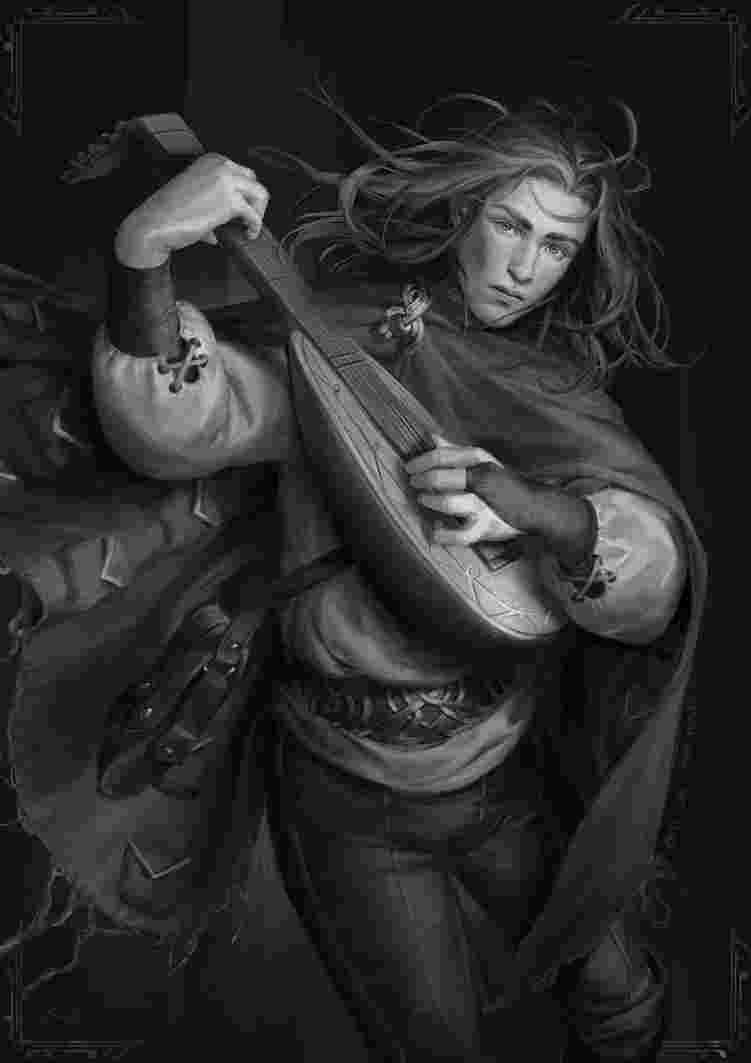
\includegraphics[width=0.24\textwidth]{./img/im4_grey}} 
    \caption{(a) RGB image (b) Greyscale image }
\end{figure}

Then it applies the Sobel operator. This consist of placing two matrices

\begin{center}
$\begin{bmatrix}
    1 & 0 & -1\\
    2 & 0 & -2\\
    1 & 0 & -1
\end{bmatrix}$ \qquad $\begin{bmatrix}
        1 & 2 & 1\\
        0 & 0 & 0\\
       -1 & -2 & -1
\end{bmatrix}$
\end{center}
in every pixel (except those on the borders) and, for each matrix. computing the sum (weighted by the matrix) of its neighbours elements. By applying each matrix, we get a measure of the variation of intensity near a pixel in the $x$ and $y$ direction. Then, we calculate the norm of the 2 dimesion vector whose components are the numbers just obtained before; that is to say, we calculate the norm of the ''intensity variation'' near each pixel. With this procedure, we get an image in greyscale where the edges are clearly marked. However, because we are using 3x3 integers matrices as the convolute operator, it is likely to happen that some lines are shown as edges when they are not. 


\begin{figure}[h!]
    \centering
    \subfigure[]{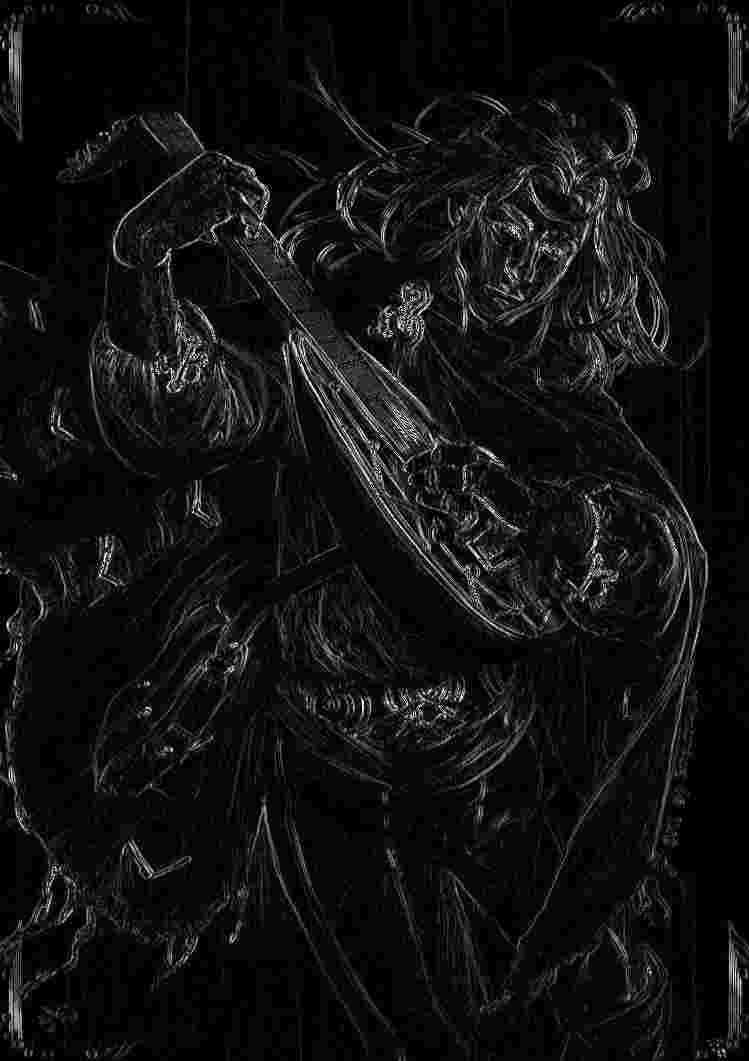
\includegraphics[width=0.24\textwidth]{./img/ejex}} 
    \subfigure[]{\includegraphics[width=0.24\textwidth]{./img/ejey}} 
    \subfigure[]{\includegraphics[width=0.24\textwidth]{./img/eje}}
    \caption{(a) Sobel in x direction (b) Sobel in y direction (c) Global Sobel}
    \label{sobel}
\end{figure}


To deal with this problem, denoising is carried out. For this part of the program, a gaussian kernel is used to ponderate the results obtained with the Sobel operator for each pixel with its local neighbours results. If a pixel mets a threshold to be considerated part of an edge, it is assigned color white and, if not, black. With this procedure, we get rid of the noise (the light blurred inside the shapes in figure \ref{sobel}) 

\myFigure{../material/img/im4_grad_denoised}{Imaged denoised}{denoised}{0.35}


\newpage
%1
\question{The program includes an outermost loop that iterates over the arguments applying the algorithms to each of the arguments (indicated as Loop 0). Is this loop optimal to be parallelized?}

It may make sense to think that this loop could be parallelized when the task we want to perform is processing a high number of images. This way, each thread would process a different image at a time.

However, this may not be the optimal approach. For example, if the images vary in size, some thread would have a lot more work to do than others, wasting resources that could help finish the task. There are other drawbacks, as explained in the next questions.

    \subquestion{What happens if fewer arguments are passed than number of cores?}
            
    The remaining cores will be idle, while the others work. This is a pretty inefficient way to distribute the tasks.

    \subquestion{Suppose you are processing images from a space telescope that occupy up to 6GB each, is this the right option? Comment how much memory each thread consumes based on the size in pixels of the input image.}

    Each thread would need to allocate memory for the RGB image and for the three new images created during the algorithm. In an RGB image, each pixel is represented with 3 bytes, one for each colour. So, if the images occupy up to 6GB, the corresponding number of pixels per image is given by: ${6\text{GB}}*\frac{2^{30}\text{B}}{1\text{GB}}*\frac{1\text{pixel}}{3\text{B}}=2^{31}\text{ pixels}$. (The program also accepts RGBA images which have an extra byte per pixel for the alpha channel).
        
    Then, each thread would need to allocate memory for the three new images it creates (grey, edges and edges\_denoised version). All of them consist of an array of bytes, one for each pixel. So it would sum up to $3\text{ grey images}*\frac{2^{31}\text{(1 channel) pixel}}{\text{1 grey image}}*\frac{1\text{B}}{\text{(1 channel) pixel}}= 6 \text{GB}$ of memory needed (apart from loading the original image of 6GB). There are other memory allocations but are insignificant when compared to the ones just commented. To sum up, every thread would need the double of memory of the image it is processing. Furthermore, this memory is freed at the end of the algorithm instead of just after where it has been used, so the total comsumption of memory of all the threads together would be even greater.


%2
\question{During the previous task (task 3), we observed that the order of access to the data is important. Are there any loops that are accessing the data in a suboptimal order? Please correct it in such case.}

    \subquestion{It is imperative that the program continue to perform the same algorithm, so only changes should be made to the program that do not change the output.}
            
    \subquestion{Explain why the order is not correct if you change it.}
    
All nested loops in \emph{main()} access data in the suboptimal order. For instance, accessing: 
\begin{equation}\label{array}
    \texttt{grey\_image[j * width + i]}
\end{equation}
This is equivalent to accessing column $i$, row $j$. Therfore, the inermost loop should iterate on $i$, accessing contiguous data in each iteration of this loop. However, the loops in the provided code do exactly the opposite, which is why we have changed them. 

In each of the nested loops inside \emph{Loop 0} we can change the order, because the instructions performed inside the innermost loop are independent from one another, which means that the order in which they are performed does not alter the result. This is similar to what we did when changing the order in which the elements were added when calculating the sum of the elements of a matrix.

In the first loop (RGB to grey scale), an element of an array is accessed in each iteration (using \ref{array}). So there is no problem.

The next loop (Sobel edge detection) does something similar, writing in array \emph{edges}. It also reads from array \emph{grey\_image}, but reading does not matter when we worry about changing order of instructions. Again, there is no alteration in the result if we change the order of this loop.

Lastly, in the \emph{denoising} filters, there is a nested loop on indices $i$ and $j$, which contains another nested loop on indices $p_1$ and $p_2$. The loops on $i$ and $j$, apart from iterating on $p_1$ and $p_2$, only write to an array: \emph{edges\_denoised}, in different positions each time. In the \emph{salt\&pepper} filter the $p_1$ and $p_2$ loops write into an array in order. This is something to take into account, as changing order in the indices would alter the result of this array; however, this array is later sorted, so the order in which it was filled is not relevant. At last, this loop can also be optimized without changing the result of the computation. In the case of the gaussian filter, the loops on indices $p_1$ and $p_2$ are used to perform an addition over the acumulator \emph{sum}; because the sum is conmutative, there is nothing to worry about. 

This improvement has been implemented in file \emph{edgeDetector\_optLoops.c}, and in all of the following parallel improvements.

%3
\question{Bypassing Loop 0, test different parallelizations with OpenMP explaining which ones should get better performance.}

    \subquestion{It is imperative that the program continue to perform the same algorithm, so only changes should be made to the program that do not change the output.}
            
We have done 3 different versions. All modifications are made to the version that uses the optimal ordering of indexes in the loops (which is written in \emph{edgeDetector\_optLoops.c}).

The first modification, \emph{par0} is such that each operation: rgb to gray, sobel transformation and gaussian denoising, has a parallelization of the outermost loop.

In the second version, \emph{par1} we have done it such that each operation has a parallelization of the outermost loop, which is forced to create 4 threads (using \texttt{num\_threads()}); and the second loop has a parallelization which is forced to create 2 threads. In total, this version creates the same number of threads ($8$) for each operation as \emph{par0}, because we are executing with the MV machine, using 8 cores.

The last version, \emph{par2}, is simillar to \emph{par0}, parallelizing the outermost loops. This time, however, we use the clause \texttt{collapse(2)}, which has been implemented speciffically to parallelize 2 nested loops of this kind: ``square loops''.

    \subquestion{It is not necessary to fully explore all the possible parallels. It is necessary to use the knowledge obtained in this task to define which would be the best solutions. Explain the reasons in the
        document.}\label{question:expected}
Of the first 2 versions, it is expected that \emph{par0} will be the best one. This is because parallelizing the outermost loop has the best results, as we have seen in exercise 3.
On the other hand, there should be no difference between \emph{par2} and \emph{par0}.

The reason why using \texttt{collapse} makes no difference relies on the number of iterations of the nested loops, in other words, the size of the image. \texttt{collpase} makes sense when the outer loop has fewer iterations than threads available (so it prevents some thread(s) from being iddle) or when the workload is uneven among iterations. But in this case, where all threads are going to be busy at all times because the number of iterations of the first loop is much higher than the number of threads, \emph{par2} and \emph{par0} are going to have similar performances.

%4
\question{Fill in a table with time and speedup results compared to the serial version for images of different resolutions (SD, HD, FHD, UHD-4k, UHD-8k). You must include a column with the fps at which the program would process}\label{question:5.4}

For obtaining the results of this exercise, we have run \emph{scr5.sh}. In order to illustrate the improvement of optimizing the index order in the nested loops, we have included the times of the original version (\emph{edgeDetector}). However, the speedups are calculated using the one with optimized loops (because we are parallelizing optimized loops).

\begin{table}[h]
    \input{./tables/table_e5_normal_times}
    \centering
    \caption{Execution time (seconds)}
\end{table}

\pagebreak

\begin{table}[h]
    \input{./tables/table_e5_normal_ratios}
    \centering
    \caption{Speedups}
    \emph{Note: in the table, speedups are calculated by columns, comparing the computations of an image with the serial version of the same image.}
    \raggedright
\end{table}

The speedup of \emph{par1} clearly grows from 1.28 to 3.02 as the image size increases.

Speedups of \emph{par2} are quite stable around 5.0-5.4. The speedups of \emph{par0} are similar, but for images SD and FHD they fall to 3.84 and 4.78, respectively. In both of this versions, we cannot clearly observe a higher speedup for larger images.

Finally, here (table \ref{fps}) we have the fps of each program and for each image size. 
\[
    \text{fps} = \text{(time in seconds per image)} ^{-1}
\]

\begin{table}[h]
    \input{./tables/table_e5_normal_fps}
    \centering
    \caption{Frames per second}
    \label{fps}
\end{table}

As expected, \emph{par0} is much better than \emph{par1} (we commented this in question \ref{question:expected}). As we also commented, \emph{par2} and \emph{par0} perfom similarly. In each of the images, the results obtained by \emph{par2} are slightly better; the difference being very small for big image sizes (UHD, 4k, 8k), and higher for smaller sized images: with a difference of a 24.3\% in the case of SD quality.

The best version, \emph{par2}, could processes images from a 
video stream in real time for videos of SD or HD definitions. If we increased the definitions of the frames, our version could not process the rate of 30 fps. In fact, for the largest resolutions, our programs cannot even process one image per second.

%5
\question{Something that we have left aside is to use compiler optimizations. Repeat the previous section adding the -O3 flag to the gcc command. Obtain information about the optimizations the compiler implements (and how they might affect our parallelization). Does the compile implement loop unrolling? Is this option activated? Does the compiler implement some kind of vectorization? Note: the -O3 option can generate warnings when compiled. Check that the output remains the same in any case.}


When the flag \emph{-O3} is included for the compilation, many optimizations are carried out; however, loop unrolling is not one of those as shown in the next image (result of adding \emph{-Q --help=optimizers} in the \emph{Makefile} to see the enabled ones). If we want the compiler to unroll loops we have to add one of these flags: \emph{-funroll-loops} or \emph{-funroll-all-loops}.

\vspace{5pt}

\lstinputlisting{tables/output_unroll}

On the other hand, the optimizations related to vectorization are the following:

\vspace{5pt}

\lstinputlisting{tables/output_vector}

Which means that some kind of vectorization is implemented. However, loop unrolling is disabled. 

In any case, the resulting images that are output by the compiled with \emph{-O3} programs are the same as the ones output by the normally compiled programs.

If we compare these results with the ones from the previous section, we notice that the average execution time has decreased by a factor of (roughly) 3 for all the versions and image resolutions. This behaviour is better observed in the fps tables: table \ref{fps} and table \ref{fps2}.


\begin{table}[h]
    \input{./tables/table_e5_O3_times}
    \centering
    \caption{Execution time (seconds) (compiling with \emph{-O3})}
\end{table}

\begin{table}[h]
    \input{./tables/table_e5_O3_ratios}
    \centering
    \caption{Speedups (compiling with \emph{-O3})}
\end{table}

This time, we can see a higher variance in the speedups of both \emph{par0} and \emph{par2}. However, \emph{par1} increases the speedup with the image size, just like in the previous question (\ref{question:5.4}).

It is also worth noting that there are images in which \emph{par0} outperforms \emph{par2}.

\begin{table}[h]
    \input{./tables/table_e5_O3_fps}
    \centering
    \caption{Frames per second (compiling with \emph{-O3})}
    \label{fps2}
\end{table}

Once again, if we only focus on the performance of the best versions; comparing this to the table from last section, we see that the fps rate has increased by a factor of 3, which would allow us to process videos in real time (30 fps) for resolutions SD, HD and FHD. However, we are still unable to process video for higher image definitions. In order to achieve so, further and more extensive parallelization would be needed as well as hardware of higher features; for instance, a larger number of cores.




\end{document}


\begin{lstlisting}[language=C, texcl=true]
    // RGB to grey scale
    int r, g, b;
    for (int i = 0; i < width; i++)
    {
        for (int j = 0; j < height; j++)
        {
            getRGB(rgb_image, width, height, 4, i, j, &r, &g, &b);
            grey_image[j * width + i] = (int)(0.2989 * r + 0.5870 * g + 0.1140 * b);
        }
    }  
\end{lstlisting}





